\documentclass[10pt,a4paper]{article}

%
% Recommended way of compilation: XeLaTeX
%

\usepackage{ifxetex}
\ifxetex
	\usepackage{fontenc}
	\usepackage{polyglossia}
	\setdefaultlanguage[variant=usmax]{english}
\else
	\usepackage[utf8]{inputenc}
\fi


\usepackage{verbatimbox}

\usepackage{framed}
\usepackage{enumerate}
\usepackage[pdfborder={0 0 0},hyperfootnotes=false]{hyperref}
\usepackage{tikz}
\usepackage{subcaption}
\usepackage{enumerate}
\usepackage{hyperref}

\usetikzlibrary{arrows,shapes,snakes,backgrounds,petri}

\title{Read Naming Format Specification}
\date{Version 0.1.1 (7 July 2015)}
\author{Karel Břinda \and Valentina Boeva \and Gregory Kucherov}

\addtolength{\textwidth}{5.4cm}
\addtolength{\hoffset}{-2.7cm}
\addtolength{\textheight}{5cm}
\addtolength{\voffset}{-3cm}

\newcommand{\re}[1]{\framebox{\mbox{\texttt{#1}}}}
\newcommand{\mre}[1]{\hspace{0.5cm}\textbf{Matching regular expression:} \re{#1}\smallskip}

\newcommand\todocit[1]{{\todo[inline,color=green!40]{#1}}}
\newcommand\todofix[1]{{\todo[inline,color=blue!40]{#1}}}

\newcommand{\RNF}{\textsc{Rnf}}
\newcommand{\SAM}{\textsc{Sam}}
\newcommand{\FASTA}{{\textsc{Fasta}}}
\newcommand{\FASTQ}{{\textsc{Fastq}}}
\newcommand{\NGS}{\textsc{Ngs}}
\newcommand{\ROC}{\textsc{Roc}}
\newcommand{\TXT}{\textsc{Txt}}
\newcommand{\HTML}{\textsc{Html}}
\newcommand{\CIGAR}{\textsc{Cigar}}

\newcommand{\SAMTOOLS}{{\textsc{SamTools}}}

\begin{document}

\maketitle


\begin{abstract}
	This document provides a standard for
	naming simulated Next-Generation Sequencing (\NGS) reads
	in order to make read simulators and mapper evaluation tools inter-compatible.
\end{abstract}


\bigskip

\begin{figure}[h]
%\centering
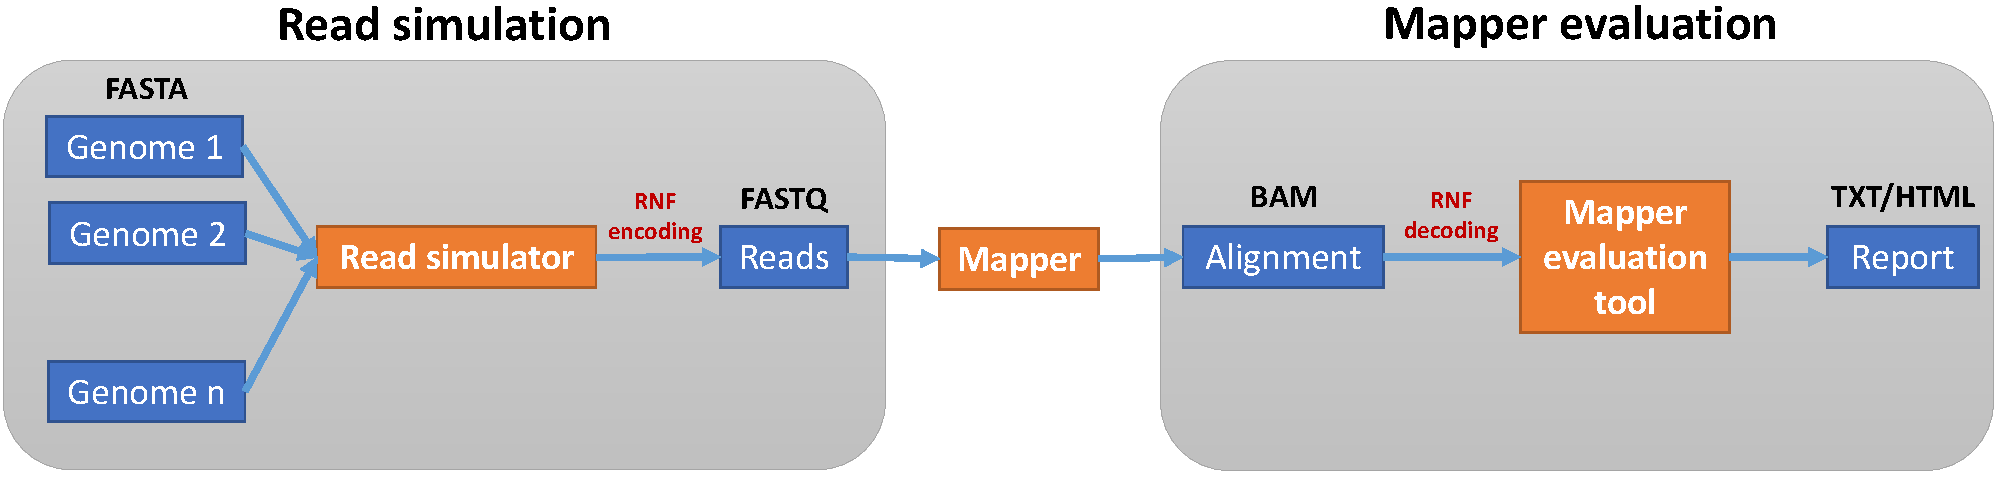
\includegraphics[width=\textwidth]{evaluation_rnf_cropped.pdf}
%\caption{
%	Evaluation of mappers of \NGS\ reads using an \RNF-compatible read simulator
%	and an \RNF-compatible alignment evaluation tool.
%	Reads are simulated from one or more genomes (some of them possibly random), mixed together.
%	After aligning them back to the reference sequence, alignments are
%	assessed by an alignment evaluation tool, which subsequently creates overall reports.
%}
\end{figure}


%%
%%
%%

\section{Terminologies and concepts}

\begin{description}
	\item \textbf{Read tuple.} 
	A tuple of sequences (possibly overlapping) obtained from a sequencing machine from a single fragment of DNA.

	\item \textbf{Reads.} 
	Members of a {\em read tuple}. For example, every ``paired-end read'' is a {\em read tuple} and both of its ``ends'' are individual {\em reads} in our notation.

	\item \textbf{Segments.}
	Substrings of a {\em read} which are spatially distinct in the reference.
	They correspond to individual lines in a \SAM\ file. Thus, each {\em read} has an
	associated chain of {\em segments} and we associate
	a {\em read tuple} with {\em segments} of all its {\em reads}.
		
	\textbf{Remarks:}
	\begin{enumerate}[-]
		\item A ``single-end read'' consists of a single {\em read} with a single {\em segment}
		unless it comes from a region with genomic rearrangment
		\item A ``paired-end read'' or a ``mate-pair read'' consists
		of two {\em reads}, each with one {\em segment} (under the same condition).
		\item A ``strobe read'' consists of several {\em reads}.
		\item A chimeric {\em read} (i.e., read corresponding to a genomic fusion, a long deletion, or a translocation) has at least two {\em segments}.
		\item Spliced reads are not considered to be spatially distinct.
	\end{enumerate}

%	\item \textbf{Read tuple name} 
	

	\item \textbf{Simulator of NGS reads.}
	A program which creates artificial simulated reads from one
	or more (possibly random) reference genomes.
	
		
	\item \textbf{Evaluation tool of NGS mappers.} 
	A program which evaluates alignments of simulated \NGS\ reads with known original
	genomic positions. It assesses if each individual read is aligned correctly. 	Finally it usually creates overall statistics.

	\item \textbf{$1$-based coordinate system.}
	A coordinate system where the first position has number $1$
	and intervals are closed (the same system is used by the \SAM\ format).
\end{description}


\begin{figure}[!tpb]
\centering

%            0         1          2         3        
\begin{subfigure}{1.0\linewidth}
\centering
\fbox{
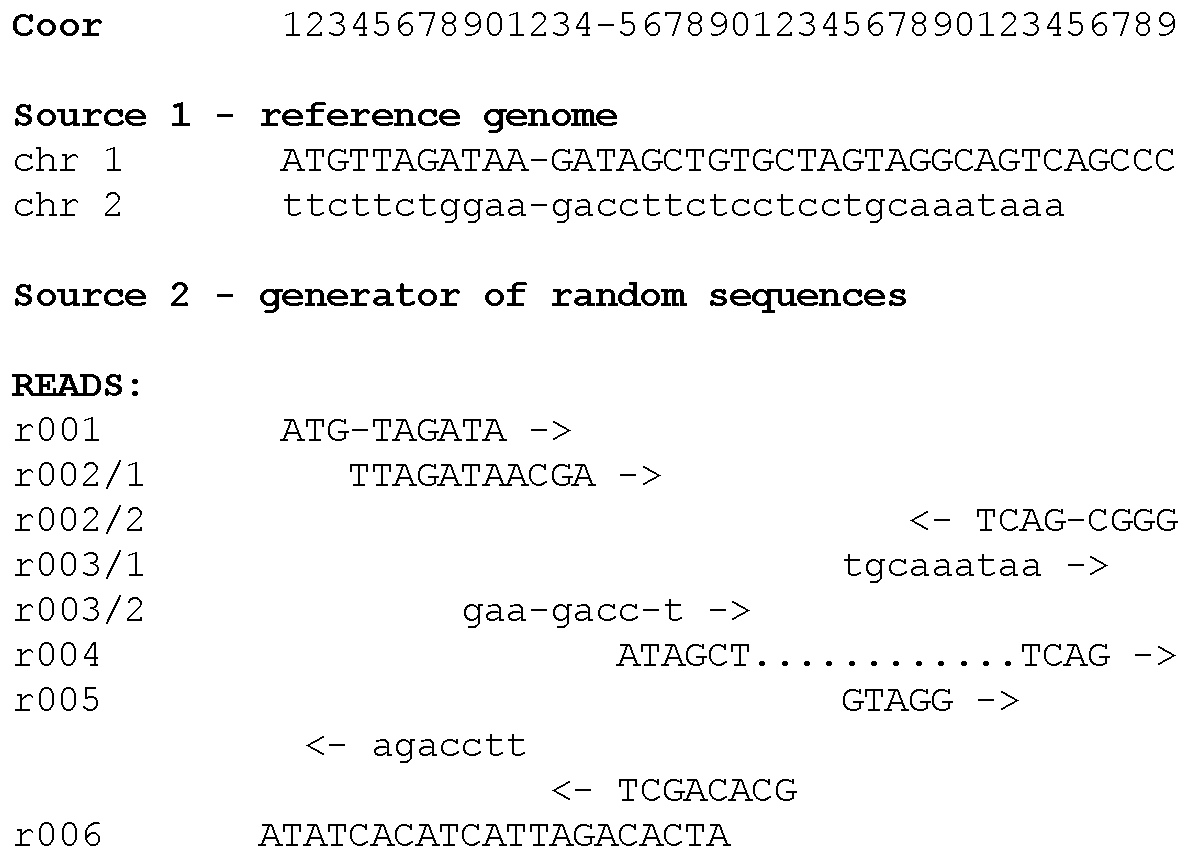
\includegraphics[width=0.6\textwidth]{rnf_example_cropped.pdf}
}

\caption{Simulated reads}
\end{subfigure}


\begin{subfigure}{1.0\linewidth}
\centering
\begin{tabular}{c|p{12.0cm}|c}
 \textbf{r. tuple} & \textbf{LRN} & \textbf{SRN} \\\hline
 r001
 	& \texttt{sim\_\_1\_\_(1,1,F,01,10)\_\_[single\_end]}
 	& \texttt{\#1}
 \\\hline
 r002
 	& \texttt{sim\_\_2\_\_(1,1,F,04,14),(1,1,R,31,39)\_\_[paired\_end]}
 	& \texttt{\#2}
 \\\hline
 r003
 	& \texttt{sim\_\_3\_\_(1,2,F,09,17),(1,2,F,25,33)\_\_[mate\_pair]}
 	& \texttt{\#3}
 \\\hline
 r004
 	& \texttt{sim\_\_4\_\_(1,1,F,15,36)\_\_[spliced],{}C:[6=12N4=]}
   	& \texttt{\#4}
 \\\hline
 r005
 	& \texttt{sim\_\_5\_\_(1,1,R,15,22),(1,1,F,25,29),(1,2,R,05,11)\_\_[chimeric]}
 	& \texttt{\#5}
 \\\hline
 r006
 	& \texttt{rnd\_\_6\_\_(2,0,N,00,00)\_\_[random]}
 	& \texttt{\#6}\\
\end{tabular}
\caption{Long and short read names}
\end{subfigure}
\caption{Example of simulated {\em read tuples} and their corresponding
Long Read Names and Short Read Names which are used
in the final \textsc{Fastq} files.
}
\end{figure}


%%
%%
%%

\section{Read tuple names}

To every {\em read tuple}, two names are assigned: {Short read name} ({SRN}) and {Long read name} ({LRN}).

\medskip

{SRN} contains a hexademical unique {\em read tuple} ID prefixed by `\texttt{\#}'.

\medskip

{LRN} consists of
four parts delimited by double-underscore:
\begin{enumerate}[i)]
	\item a prefix (possibly containing expressive 
information for a user or a particular string
for sorting or randomization of order of tuples),
	\item the {\em read tuple} ID,
	\item information about origins of all {\em segments} that constitute {\em reads} of the {\em tuple},
	\item a suffix containing arbitrary comments or extensions (for holding additional information).
\end{enumerate}


\medskip

Preferred final read names are {LRNs}. If an {LRN} exceeds $255$ (maximum allowed read length in 
\SAM), 
{SRNs} are used instead and a SRN--LRN correspondence file must be created. 



%%
%%

\subsection{Read tuple ID}

It is a positive integer, which is unique within a single file with genomic data.
These IDs are assigned continuously from $1$. Zero is reserved for ``not available''.


%%
%%

\subsection{SRN -- Short Read Name}
\mre{\char92\char35([0-9a-f]+)}.

{SRN} consists of {\em read tuple} ID prefixed by
`\texttt{\#}'.
It is displayed as zero padded hexadecimals in lowercase such 
that all {SRN}s share the same string
length within a single file.


%%
%%

\subsection{LRN -- Long Read Name}
\mre{\char94([\char33-\char63\char65-\char94\char96-\char126]*)\_\_([0-9a-f]+)\_\_([\char33-\char63\char65-\char94\char96-\char126]+)\_\_([\char33-\char63\char65-\char94\char96-\char126]*)\char36}.

{LRN} consists of four double-underscore-delimited parts:
i)~{prefix part},
ii)~{\em read tuple} ID,
iii)~ {segmental part},
iv)~{suffix part}.



%%
%%

\label{prefix_part}
\subsection*{Prefix part}
\mre{\char94[\char33-\char63\char65-\char94\char96-\char126]*\char36}

It can be an empty string, a string containing
expressive ``visual'' information for the user
(e.g., for easy distinguishing random reads from the others),
or a string used for randomization of {\em read tuples} (randomly taken prefix and {\em read tuples} sorted in lexicographical order).

Length of all prefix parts within a single file must be equal.



%%
%%

\label{readid_part}
\subsection*{Read tuple ID part}
\mre{\char94[0-9a-f]+\char36}

It displays {\em read tuple} ID as hexadecimals
in lowercase. All {\em read tuple} ID parts are zero padded such that
they all share the same string length within a single file.


%%
%%

\subsection*{Segmental part}\label{segmental_part}

\mre{\char94(?:(\char92([0-9FRN,]*\char92))(?:,(?!\char36)|\char36))+\char36}

{Segmental part} consists of one or more comma-delimited {segments}.

%

\subsubsection*{Segment}

\mre{\char94\char92(([0-9]+),([0-9]+),([FRN]),([0-9]+),([0-9]+)\char92)\char36}

Every {segment} is parenthesized and consists
of five comma-delimited values:
i) {genome ID},
ii) {chromosome ID},
iii) {direction},
iv) {leftmost coordinate}, and
v) {rightmost coordinate}.

\medskip

\begin{tabular}{|p{3.4cm}|p{11.0cm}|}
\hline
	{Genome ID} &
		ID (positive integer) of the source genome
		(a randomly generated genome, a genome saved in a \FASTA\ file,
		etc.) or zero for ``not available''. 
		\newline\newline
		All numbers of genomes are displayed as decimals and they
		are zero padded such that
		they all share the same string length within a single file. 
		\\\hline
	{Chromosome ID} &
		ID (positive integer) of the source chromosome
		or zero for ``not available''.
		\newline
		\newline
		All numbers of chromosomes are displayed as decimals and they are zero padded such that they all share the same string length within a single file.
		\newline
		\newline
		IDs are assigned continuously from $1$,
		order chromosomes is the same as in
		the file, where the genome is saved.
		In case of a random genome, zero should be used.
		\\\hline
	{Direction} &
		Direction in the reference genome.
		\newline
		\newline
		`F' = forward direction \newline
		`R' = reverse direction \newline
		`N' = not available
		\newline
		\newline
		For random reads, `N' should be used.
		\\\hline
	{Leftmost coordinate} &
		The leftmost
		coordinate of the segment in the reference in 1-based coordinate system or zero for ``not available''. 
		\\\hline
	{Rightmost coordinate} & 
		The rightmost
		coordinate of the segment in the reference in 1-based coordinate system or zero for ``not available''. 
		\\\hline
\end{tabular}



%%
%%

\label{suffix_part}
\subsection*{Suffix part}
\mre{\char94(?:((?:[a-zA-Z0-9]+:)\char123{}0,1\char125)\char92[([\char33-\char63\char65-\char90\char92\char92\char94\char96-\char126]*)\char92](?:,(?!\char36)|\char36))+\char36}

It contains arbitrary number of comma-delimited
{comments} and {extensions} in
any order.


%%

\subsubsection*{Comment}
\mre{\char94[([\char33-\char63\char65-\char90\char92\char92\char94\char96-\char126]*)]\char36}

{Comments} are displayed as square-bracketed strings.
They can contain, e.g., information
about the simulated technology or the program used for
simulation.

%%

\subsubsection*{Extension}
\mre{\char94([A-Za-z0-9]+):\char92[([\char33-\char63\char65-\char90\char92\char92\char94\char96-\char126]*)\char92]\char36}

An {extension} consist of an {extension's code}, a colon, and
a square-bracketed {extension's content}.
Extensions can supplement the basic set of information provided in segmental part.
Some of them are part of this standard,
see Section~\ref{sec:extensions}.


%%
%%
%%

\section{SRN--LRN correspondence file}
\label{sec:correspondence_file}

To encode information about correspondence between
SRN and LRN,
a special file is created. Its file name is formed of
prefix of the \FASTQ\ file(s) and
\texttt{.sl} suffix.

\medskip

Examples:
\smallskip

\begin{tabular}{l|l}
	Read files & SRN-LRN correspondence file \\\hline
	\texttt{reads\_se.fq} & \texttt{reads\_se.sl} \\
	\texttt{reads\_se.fastq} & \texttt{reads\_se.sl} \\
	\texttt{reads\_pe.1.fq}, \texttt{reads\_pe.2.fq} & \texttt{reads\_pe.sl}
\end{tabular}

\smallskip

It is a
tab delimited file with two columns (containing SRN and the corresponding LRN). File is sorted by {\em read tuple} ID.


%%
%%
%%

\section{Extensions}
\label{sec:extensions}
\appendix

Extensions can supplement the basic set of information provided in the segmental part (Section \ref{segmental_part}).

\subsection*{C -- CIGAR strings}

\subsubsection*{Extension's code}

\hspace{0.5cm} C

\subsubsection*{Extension's content}

\mre{\char94(?:([0-9]+[=XIDNSHPM]+)(?:,(?!\char36)|\char36))+\char36}


\subsubsection*{Specification}

The extension can be used to encode edit operations 
using \CIGAR\  (Compact Idiosyncratic Gapped Alignment Report) strings.

\medskip

\begin{table}[h]
\centering
\caption*{Supported operations:}
\begin{tabular}{|l|l|p{8cm}|}
	\hline
	letter & operation & comment 
	\\\hline
	\texttt{=} & match & \\
	\texttt{X} & mismatch & \\
	\texttt{I} & insertion & \\
	\texttt{D} & deletion &	\\
	\texttt{N} & skipping bases & skipping intron regions in spliced mapping \\
	\texttt{S} & soft clipping &
		for cutting unaligned prefixes and suffixes \\
	\texttt{H} & hard clipping &
		for cutting unaligned prefixes and suffixes \\
	\texttt{P} & padding & unused padding in padded reference\\
	\texttt{M} & match or mismatch	& deprecated, reserved for situations when distinguishing \texttt{X} vs. \texttt{=}
is impossible
	\\\hline
\end{tabular}
\end{table}

\medskip

\CIGAR\ strings should be provided in the same order as their corresponding segments in the {segmental part} (Section \ref{segmental_part}). Adjacent edit operations should be different.

\subsubsection*{Example}

\begin{framed}\small
\begin{verbatim}
	demonstration__004__(1,1,F,16,40),(1,1,R,140,150)__C:[6=14N5=,11=],[spliced_paired_end_read]
\end{verbatim}
\end{framed}




%%
%%
%%

\begin{thebibliography}{}
	\bibitem{samtools}
	Li, H. \textit{et al.} (2009)
	The Sequence Alignment/Map format and SAMtools.
	\textit{Bioinformatics} \textbf{25}(16): 2078--2079.
\end{thebibliography}


\end{document}

